%\yoc{I strengthened this section towards discussing why the things we consider are important. }
In this section, we explain information about the test problems in summarized manner. This includes problem origin, type, components (variables and constraints), and sparsity for each problem. We explain why they are important for advances in SIP research study. This section reflects our philosophy in developing \siplibtwo. Detailed problem-specific information is available in Section \ref{sec:prob_desc} for those who are interested in.

\subsection{Origin of the problems}
Table \ref{table:problems} summarizes the description of each test problem in \siplibtwo. The five of them are adopted from \siplib\ \cite{web:SIPLIB1}. We tried to implement the \siplib\ instances as the same as the original references possible. Not all of them, however, are exactly the same due to insufficient information on some parameters. We needed to guess the missing links and sometimes develop our own way to implement the problems. 
\begin{table}[H]
	\centering
%	\resizebox{\textwidth}{!}{%
			\caption{Problems in \siplibtwo}
			\label{table:problems}
			\begin{tabular}{@{}llll@{}}
				\toprule
				Problem		  		  & Description                                                        & Main reference              \\ \midrule
				\dcap\         & \makecell[tl]{Dynamic capacity planning with stochastic\\ demand (\ref{DCAP}) }                  & Ahmed and Garcia \cite{journal:AG2004}                          \\
				\mptsps\       & \makecell[tl]{Multi-path traveling salesman problem with\\ stochastic travel costs (\ref{MPTSPs})}& Tadei et al. \cite{journal:TPP2017}                            \\
				\sizes\        & \makecell[tl]{Optimal product substitution with stochastic\\ demand (\ref{SIZES})}         & Jorjani et al. \cite{journal:JSW1999}          \\
				\smkp\		  & Stochastic multiple knapsack problem (\ref{SMKP})                              & Angulo et al. \cite{journal:AAD2014}                            \\
				\sslp\         & Stochastic server location problem (\ref{SSLP})                                & Ntaimo and Sen \cite{journal:NS2005}                           \\
				\suc\         & Stochastic unit commitment problem	(\ref{SUC})			               & Papavasiliou and Oren \cite{journal:PO2013}                       \\ \bottomrule
			\end{tabular}%
			
			%			\begin{tablenotes}
			%				\small
			%				\item For convenience, we skip the cardinality sign $|\cdot|$ for sets, i.e., for any set $S$, $S$ denotes the number of elements $|S|$ in this table.
			%			\end{tablenotes}
%	}
\end{table}

\subsubsection{How we deal with missing links and errors}
%\yoc{This subsection is newely added to discuss the issues on implementaion.}
During implementation, we often have faced some missing links and errors. The missing links are largely from the two parts: data generation and instance parameters. For example, we could not catch the exact data generating procedure for \mptsps\ even after looking up all the references. For \sslp, the parameters for the zonal constraints are not provided ($Z$, $w_z$, $J_z$ in Table \ref{sslp:notation}). 

We also found some errors. The errors are not critical so the accompanied instances are still solvable somehow. The result, however, might be different from the originally intended. For example, the big-M constant in the logical constraint (\ref{dcap:b}) in \dcap\ is set to be 1 rather than suitably large value in the \smps\ files. For \sslp, the redundant constraint (\ref{sslp:b}) presents in the \smps\ files. 

We set the following rule to address such issues described above.
\begin{enumerate}
	\item Follow the original implementation including the errors whenever we are able to reproduce it.
	\item Develop our own way as long as it does not harm the endemic characteristic of the problem.
\end{enumerate}

The notable remark for each problem briefly presents in Table \ref{table:remarks}.
\begin{table}[H]
	\centering
%	\resizebox{\textwidth}{!}{%
		\begin{threeparttable}
			\caption{Implementation remarks for each problem}
			\label{table:remarks}
			\begin{tabular}{@{}llp{3in}}
				\toprule
				Problem & \multicolumn{1}{c}{Remark}                                                \\ \midrule
				\dcap   & We go with the error in constraint (\ref{dcap:b})                                              \\
				\mptsps & \makecell[tl]{We adopt formulation from another reference \cite{journal:LSD1990}, We develop data \\generation procedure \ref{mptsps:datagen}} \\
				\sizes  & We modify the formulation to polish (\ref{sizes:obj})-(\ref{sizes:h})                                                    \\
				\smkp   & -                                                                         \\
				\sslp   & \makecell[tl]{We keep the zonal components empty and let the redundant constraint (\ref{sslp:b})\\ present }                                    \\
				\suc    & We generate and provide up to 1,000 stochastic wind scenario data                                    \\ \bottomrule
			\end{tabular}
			\begin{tablenotes}
				\small
				\item - means no issue presents
			\end{tablenotes}
		\end{threeparttable}
%	}
\end{table}

\subsection{Instance naming rule}
Table \ref{table:naming_rule} shows how we name the instances. We change the original naming convention for consistency and future extension. Some legacy naming rules do not consider the case when the set cardinality becomes larger than 1 digit number. Moreover, since some \siplibtwo\ instances can be generated using more sets other than used in \siplib, we needed to define a new naming convention. For example, we change the instance names of \dcap\ and \smkp\ as below.
\begin{quote}
	\centering dcap$RNT$\_$\mathcal{S}$ $\longrightarrow$ DCAP$\_R\_N\_T\_\mathcal{S}$\\
	smkp$\_\mathcal{S}$ $\longrightarrow$ SMKP$\_I\_\mathcal{S}$
\end{quote}
For \dcap, we just add underbars ``\_'' to delimit set cardinalities. Without delimiter, the instance name causes confusion when set cardinality is greater than or equal to 10. For \smkp, we add new set cardinality $I$ since the fixed number $|I|=120$ can be changed by user if desired.

The capital Roman letters mean the sets defining the problems. In particular, the calligraphic letter $\mathcal{S}$ always denotes the scenario set. For notational convenience, we sometimes skip the cardinality sign $|\cdot|$ for sets, i.e., for set $S$, $S$ itself denotes the number of elements $|S|$ in Table \ref{table:naming_rule} and \ref{table:num_components}. Note that not all sets are used to define an instance. The sets that do not appear in the instance name are fixed by some pre-determined value by the original references so we follow them. For example, in \smkp\ there are four sets in total, $I,J,K,\mathcal{S}$, but the numbers of knapsacks $|J|$ and $|K|$ are fixed by 50 and 5 so do not appear in the instance name.
\begin{table}[H]
	\centering
	\caption{Instance naming rules}
	\label{table:naming_rule}
	\resizebox{\textwidth}{!}
	{%
		\begin{tabular}{@{}llp{3in}}
			\toprule
			Problem & Instance name                 & \multicolumn{1}{c}{Remark}                                                                    					      \\ \midrule
			\dcap\    & DCAP\_$R$\_$N$\_$T$\_$\mathcal{S}$    &   $R$: number of resources, $N$: number of tasks, $T$: number of time periods, $\mathcal{S}$: number of scenarios        \\
			\mptsps\  & MPTSPs\_$D$\_$N$\_$\mathcal{S}$ &$D$: node distribution strategy, $N$: number of nodes, $\mathcal{S}$: number of scenarios\\
			\sizes\   & SIZES\_$\mathcal{S}$                            & $\mathcal{S}$: number of scenarios   															\\
			\smkp\    &   SMKP\_$I$\_$\mathcal{S}$    &   $I$:number of types for item, $\mathcal{S}$: number of scenarios  													 \\
			\sslp\    &  SSLP\_$I$\_$J$\_$\mathcal{S}$      &    $I$: number of clients, $J$: number of server locations, $\mathcal{S}$: number of scenarios                 				   \\
			\suc\    & 	SUC\_$D$\_$\mathcal{S}$    &  $D$: day type, $\mathcal{S}$: number of scenarios                                                 						 \\ \bottomrule
		\end{tabular}%
	}
\end{table}

\subsection{Type of the problems}
In \siplibtwo\, we mainly classify each problem by its stage-wise variable types. Many decomposition-based solution methods in SIP require specific type of variables to be presented in each stage, e.g., \cite{journal:LL1993,journal:SSV1998,journal:CT1998,journal:CS1999,journal:SF2002}. They oftentimes exploit the characteristics of the variables to extend the former decomposition methods developed for NLP, LP, IP, and MIP. Therefore, the stage-wise variable type is one of the most important factor to classify SIP problems.

We consider three types of variable: continuous, binary, and integer. Considering two stages, the possible number of combination is $\left[\sum_{k=1}^3\binom{3}{k}\right]^2=49$ in total. We try to include problems with non-overlapping such combination. Table \ref{table:prob_class} shows the stage-wise components (variable and constraints) of each problem. For the abbreviated notation on the constraints, we refer to \miplib\ \cite{MIPLIB}. Although the constraint type is possibly one of the important factors that define the problem characteristic, we decided not to consider it for classification since it can cause too much variety, i.e., different problem contains different constraints, which we cannot easily capture the insight from the problem type classification. 
\begin{table}[H]
	\centering
	\caption{Components of the problems}
	\label{table:prob_class}
	\begin{threeparttable}
		\begin{tabular}{@{}lllll@{}}
			\toprule
			& \multicolumn{2}{c}{1st stage}                              				  	& \multicolumn{2}{c}{2nd stage}                             			        \\ \midrule
			Problem 	     & Variable                    & Constraint                   	& Variable                    & Constraint                  				    \\ \midrule
			\dcap\ (\ref{dcap:formulation})    & $\mathbb{C}$, $\mathbb{B}$  & \texttt{VBB}                	& $\mathbb{B}$                & \texttt{PAR}, \texttt{M01} 			    		\\
			\mptsps\ (\ref{mptsps:formulation})  & $\mathbb{C}$, $\mathbb{B}$  & \texttt{PAR}, \texttt{GEN}		& $\mathbb{B}$                & \texttt{GEN}               						\\
			\sizes\ (\ref{sizes:formulation})   & $\mathbb{I}$ 			   & \texttt{VBD}, \texttt{GEN} 	& $\mathbb{B}$, $\mathbb{I}$  & \texttt{IKN}             						\\
			\smkp\ (\ref{smkp:formulation})   & $\mathbb{B}$                & \texttt{KNA}                	& $\mathbb{B}$                & \texttt{KNA}              						\\
			\sslp\ (\ref{sslp:formulation})   & $\mathbb{B}$                & \texttt{IVK}, \texttt{GEN} 	& $\mathbb{C}$, $\mathbb{B}$  & \texttt{GEN}             						\\
			\suc\ (\ref{SUC:formulation})   & $\mathbb{C}$, $\mathbb{B}$                 & \texttt{VBB}, \texttt{GEN}                            	& $\mathbb{C}$, $\mathbb{B}$  &  \texttt{VBB}, \texttt{GEN}                                  					\\ \bottomrule
		\end{tabular}
		
		\begin{tablenotes}
			\small
			\item *$\mathbb{C}$: continuous, $\mathbb{B}$: binary, $\mathbb{I}$: integer
			\item **Constraint type notation is adopted from \texttt{MIPLIB 2010}. Refer to the tables in Section \ref{sec:miplibconstraint}.
		\end{tablenotes}
	\end{threeparttable}
\end{table}

\subsection{Number of components}
Table \ref{table:num_components} summarizes the number of components (variables and constraints) in each problem from \siplibtwo. The numbers can be calculated based on the cardinality of the sets that define the problems.

Although no universally effective way to measure the difficulty of MIP is discovered yet, the number of components in instance is one of the closely related factor. For example, instances tend to be more difficult as the number of discrete variables increases. The continuous variables, which hardly are problematic when solely present by themselves, can also let the instance burdensome when mixed with integer variables. 

The increase in the number of constraint, although not always, is an important factor that difficultize the instance. This affects every iteration from the LP relaxation given the requirement of inverting a matrix for every basic feasible solution visited in the process. We investigate the number of components present in instance. For those who want to generate instances with some desired number of components can utilize Table \ref{table:num_components}.
\begin{table}[H]
	\centering
	\resizebox{\textwidth}{!}{%
		\begin{threeparttable}
			\caption{Number of components in each problem}
			\label{table:num_components}
			\begin{tabular}{@{}lccccc@{}}
				\toprule
				&               & \multicolumn{4}{c}{Components}                                                                         \\ \cmidrule(l){3-6} 
				&                & \#Continuous   & \#Binary                           & \#Integer            & \#Constraint              \\ \midrule
				\multirow{3}{*}{\dcap\ (\ref{dcap:notation})}   & 1st stage & $RT$           & $RT$                               & -                    & $RT$                      \\
				& 2nd stage & -             & $(1+R)NT$               & -                    & $(R+N)T$                  \\ \cmidrule(l){2-6} 
				& Total          & $RT$           & $RT+(1+R)NTS$ & -                    & $RT+(R+N)T\mathcal{S}$    \\ \midrule
				\multirow{3}{*}{\mptsps (\ref{mptsps:notation})} & 1st stage & $(N-1)N$          & $(N-1)N$                              & -                    & $N^2+2N-1$                \\
				& 2nd stage & -              & $3(N-1)N$                            & -                    & $(N-1)N$                     \\ \cmidrule(l){2-6} 
				& Total          & $(N-1)N$          & $(N-1)(1+3\mathcal{S})N$              & -                    & $(1+\mathcal{S})N^2+(2-\mathcal{S})N-1$ \\ \midrule
				\multirow{3}{*}{\sizes\ (\ref{sizes:notation})}  & 1st stage & -              & $2N$                               & $2N$                 & $2(1+N)$                  \\
				& 2nd stage & -              & -                                  & $N(N+1)$              & $4N$                     \\ \cmidrule(l){2-6} 
				& Total          & -              & $2N$                               & $2N+N(N+1)\mathcal{S}$ & $2(1+N+2N\mathcal{S})$    \\ \midrule
				\multirow{3}{*}{\smkp\ (\ref{smkp:notation})}   & 1st stage & -              & $2I$                               & -                    & $J$                       \\
				& 2nd stage & -              & $I$                                & -                    & $K$                       \\ \cmidrule(l){2-6} 
				& Total          & -              & $(2+\mathcal{S})I$                 & -                    & $J+K\mathcal{S}$          \\ \midrule
				\multirow{3}{*}{\sslp\ (\ref{sslp:notation})}   & 1st stage & -              & $J$                                & -                    & $1$                       \\
				& 2nd stage & $J$            & $IJ$                               & -                    & $I+J$                     \\ \cmidrule(l){2-6} 
				& Total          & $J\mathcal{S}$ & $(1+I\mathcal{S})J$                & -                    & $1+(I+J)\mathcal{S}$      \\ \midrule
				\multirow{3}{*}{\suc\ (\ref{SUC:notation})}   & 1st stage & 960               &   1000                                 &     -                 &  2208                         \\
				& 2nd stage & 21274               &     2250                               &   -                   & 24780                          \\ \cmidrule(l){2-6} 
				& Total          & $960+21274\mathcal{S}$                &  $1000+2250\mathcal{S}$                                  &  -                    &  $2208+24780\mathcal{S}$                         \\ \bottomrule
			\end{tabular}
			
			\begin{tablenotes}
				\small
				\item *For convenience, we skip the cardinality sign $|\cdot|$ for sets.
				\item **We insert numerical value for the predetermined set, e.g., for \sizes, we use $|T|=2$ and for \mptsps, we use $|K_{ij}|=3$. In \suc, all the sets are predetermined based on the given data except for the scenario set $\mathcal{S}$.
			\end{tablenotes}
		\end{threeparttable}
	}
\end{table}

\subsection{Sparsity} \label{subsec:sparsity}
As can be seen in Fig \ref{fig:stagewise_sparsity}, there are three differently structured blocks in EF. Every other block is the duplication of block T or W hence the same sparsity pattern repeats as many as the number of scenarios considered. Block A and W are only related with their own stage while block T is related with both. Block T is called \textit{technology}  matrix. In section \ref{sec:sparsity} in the appendix, we report tables providing block-wise sparsity that is derived solely based on the set cardinality.
\begin{figure}
	\centering
	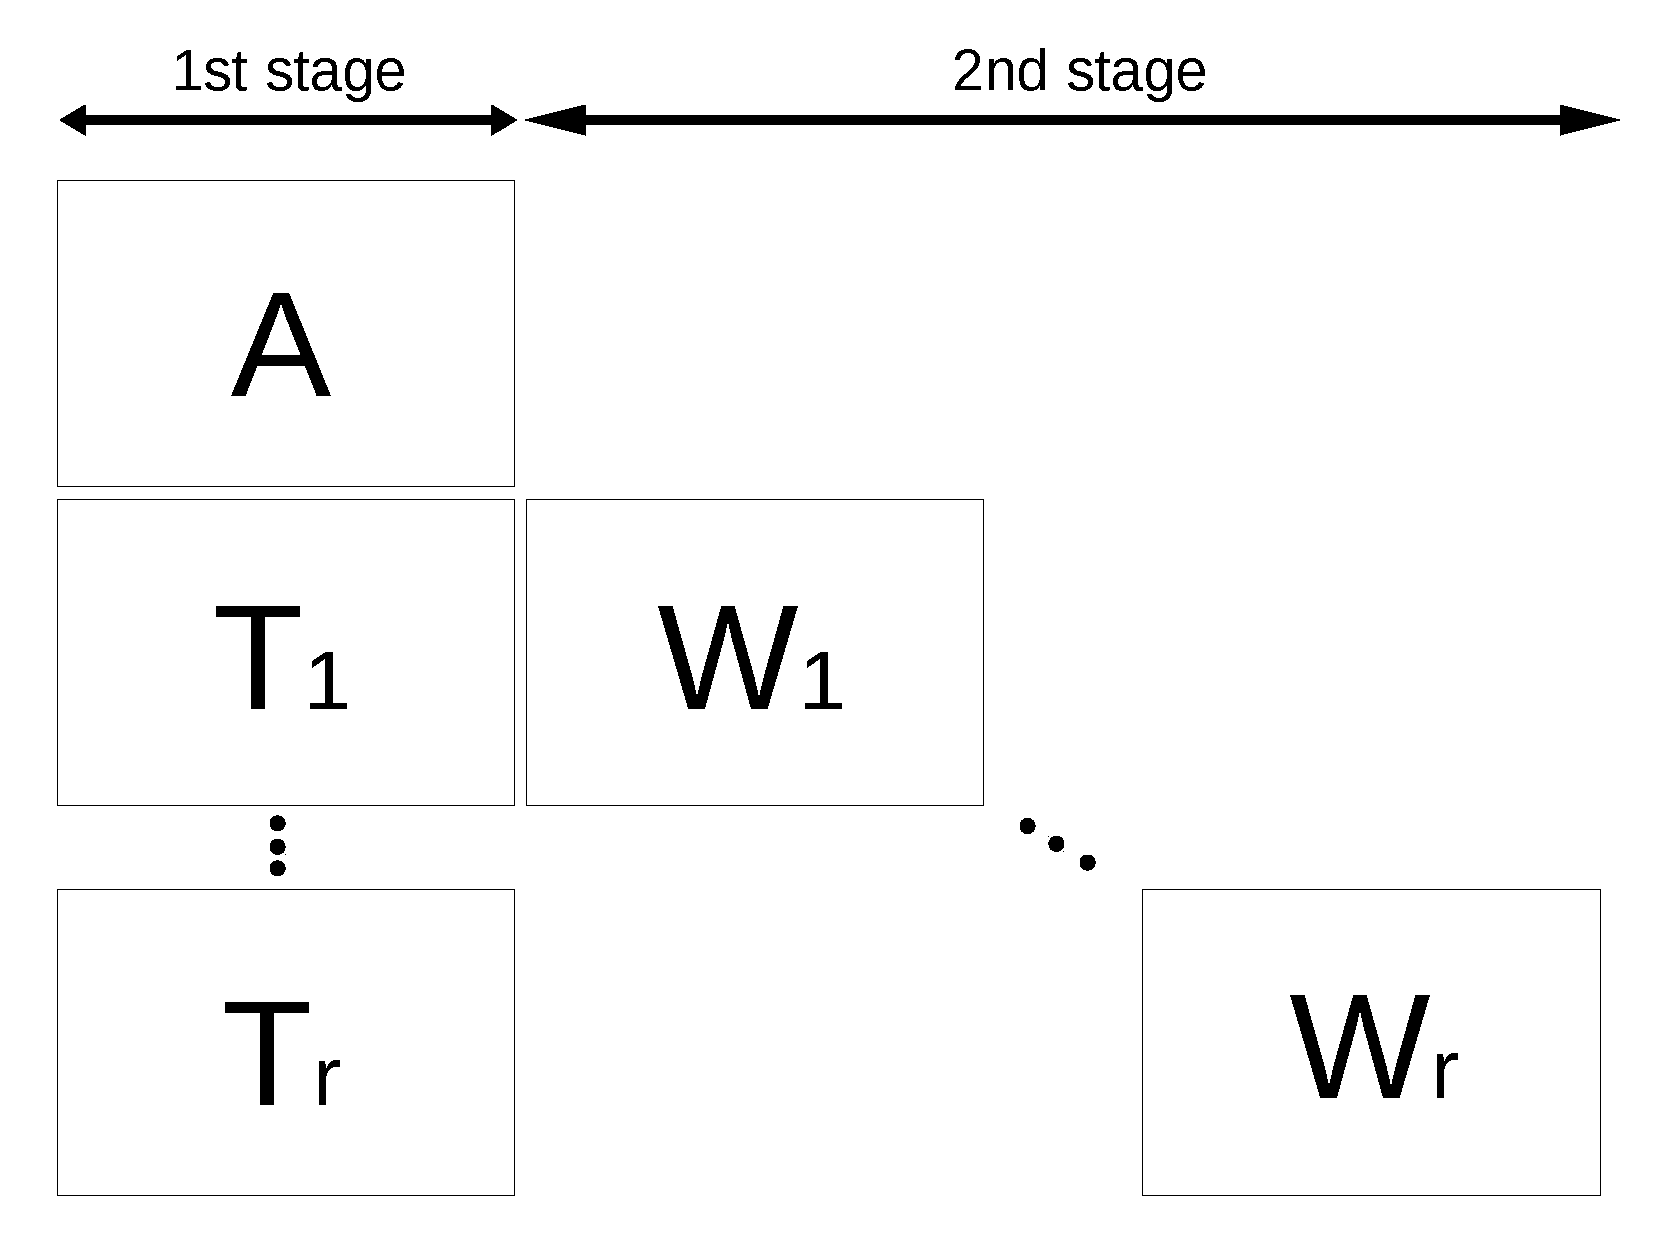
\includegraphics[width=0.7\linewidth]{drawings/stagewise_sparsity}
	\caption{Three (structurally) independent blocks in SIP}
	\label{fig:stagewise_sparsity}
\end{figure}

Every SIP in EF has a block-diagonal structure in its coefficient matrix (Fig \ref{fig:de_structure}). This characteristic differentiates SIP from the general MIP. In particular, the block-diagonal structure results always in high sparsity as scenario increases. Hence, it does not seem to be meaningful to just report the sparsity of the extensive form coefficient matrix.
\begin{figure}[]
	\centering
	\subfloat[][DCAP\_3\_3\_3\_3]
	{
		\centering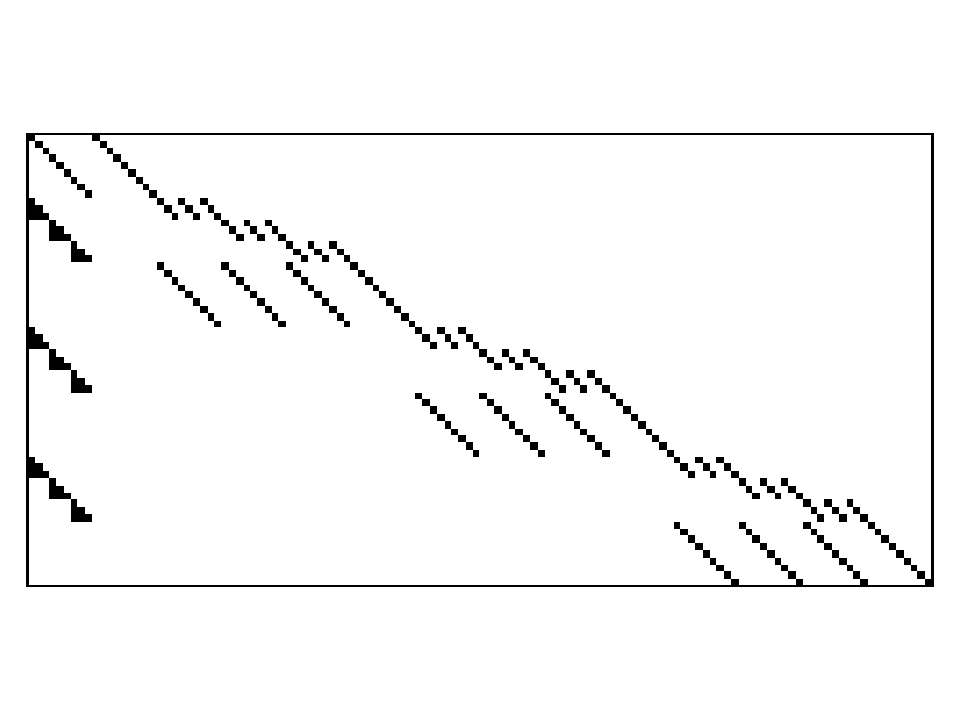
\includegraphics[width=0.45\linewidth]{DCAP_3_3_3_3}
		\label{fig:de_structure_dcap}
	}
	~
	\subfloat[][MPTSPs\_D0\_3\_3]
	{
		\centering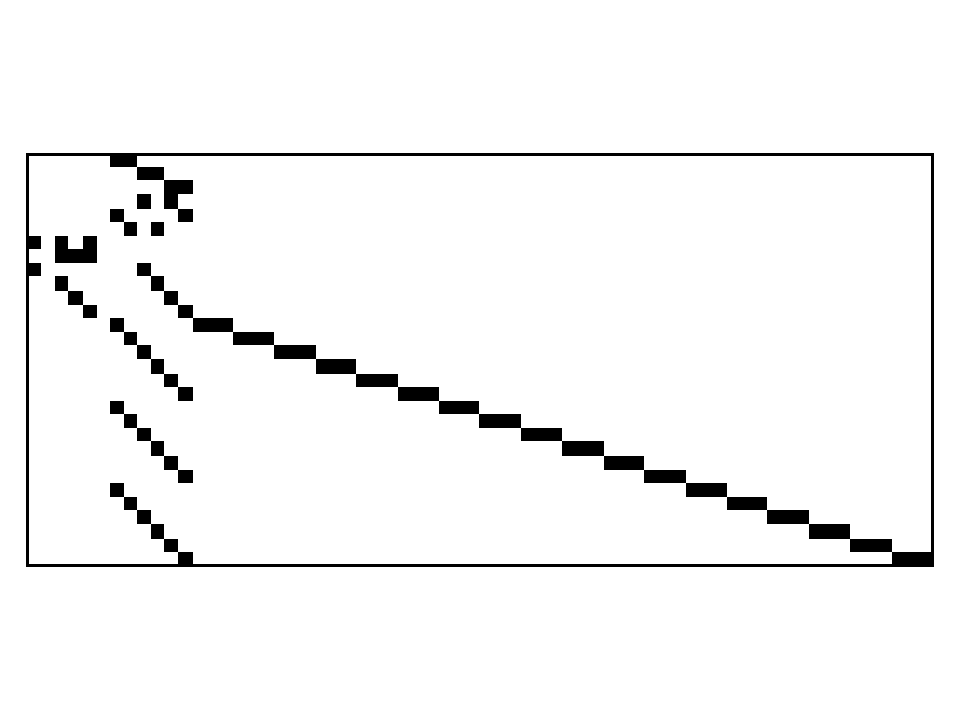
\includegraphics[width=0.45\linewidth]{MPTSPs_D0_3_3}
		\label{fig:de_structure_mptsps}
	}
	
	\subfloat[][SIZES\_3]
	{
		\centering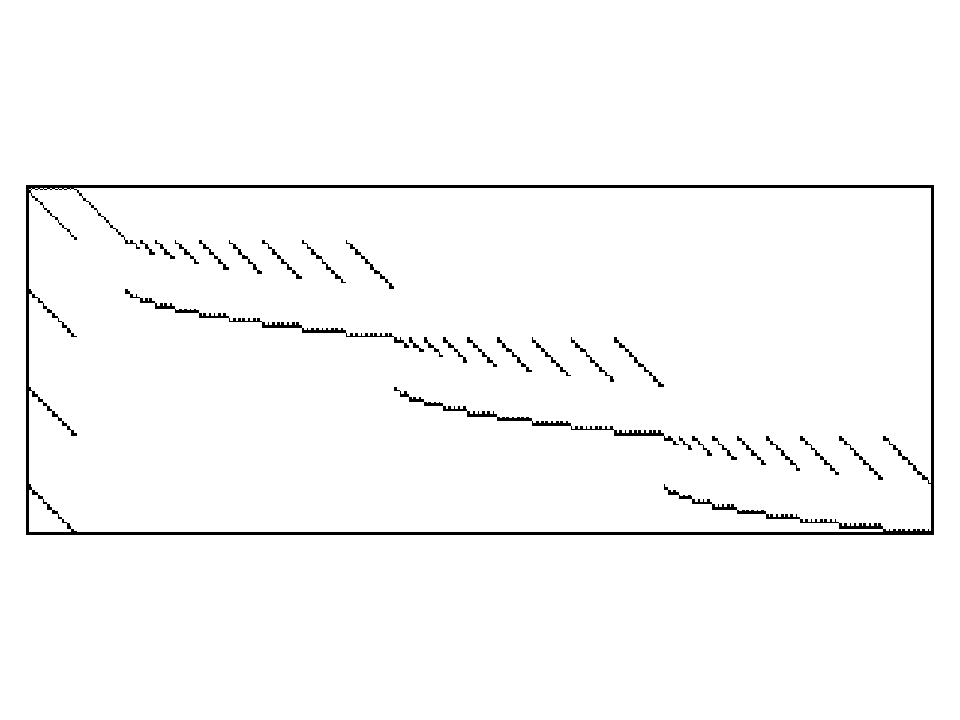
\includegraphics[width=0.45\linewidth]{SIZES_3}
		\label{fig:de_structure_sizes}
	}
	~
	\subfloat[][SMKP\_120\_3]
	{
		\centering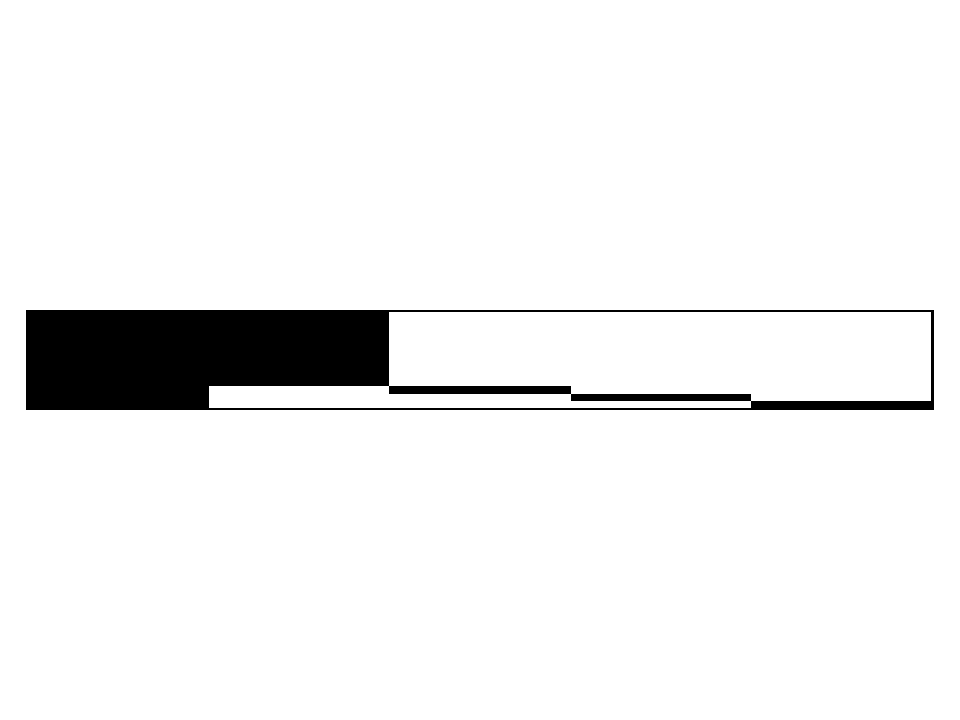
\includegraphics[width=0.45\linewidth]{SMKP_120_3}
		\label{fig:de_structure_smkp}
	}
	
	\subfloat[][SSLP\_5\_10\_3]
	{
		\centering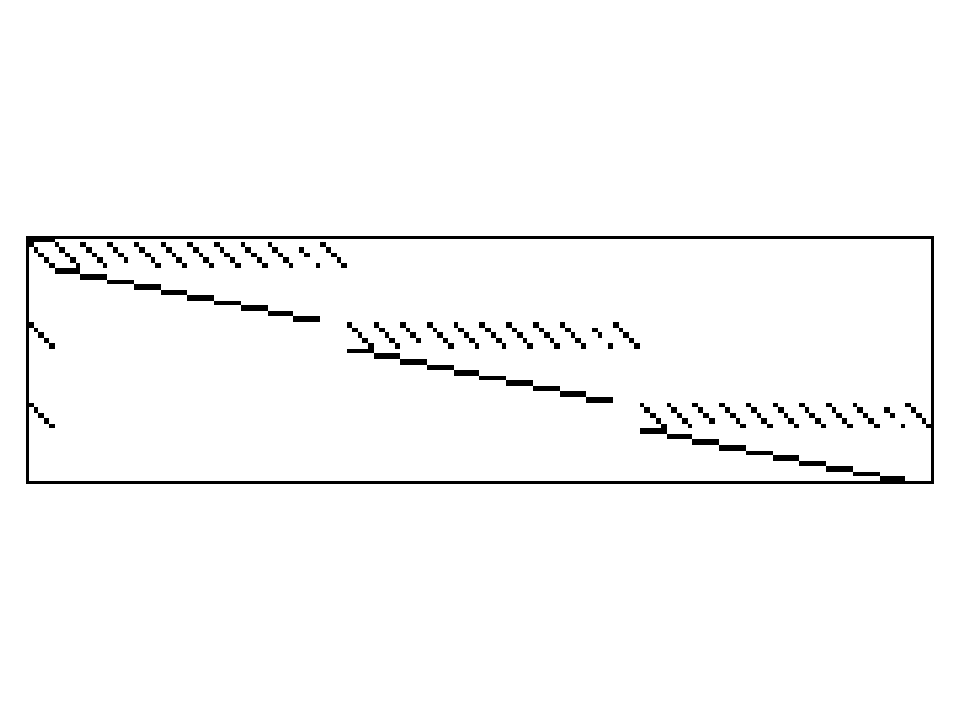
\includegraphics[width=0.45\linewidth]{SSLP_5_10_3}
		\label{fig:de_structure_sslp}
	}
	~
	\subfloat[][SUC\_FallWD\_1]
	{
		\centering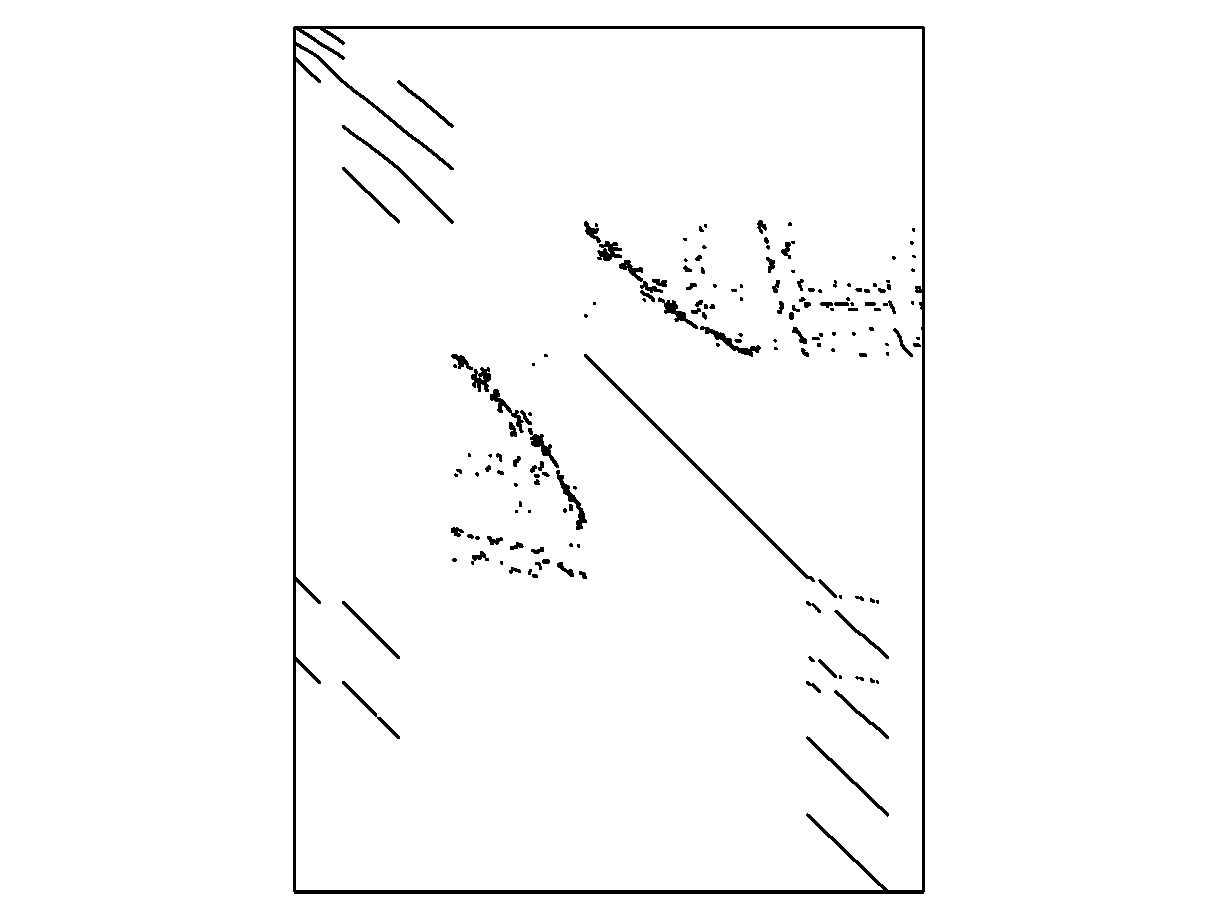
\includegraphics[width=0.45\linewidth]{SUC_FallWD_1}
		\label{fig:de_structure_sucw}
	}
	
	\caption{Block-diagonal structure in extensive form}
	%	\begin{minipage}
	%		{0.65\textwidth}{\footnotesize *\suc\ instance is too huge and extremely sparse to plot more than 1 scenario}
	%	\end{minipage}
	\label{fig:de_structure}
\end{figure}

As many decomposition-based methods in SIP make use of solution methods developed for MIP to solve the descendant master/sub problems, exploiting the sparsity pattern in each independent block might be one of the key aspects that will help improving performance of the algorithms. Given the sparsity pattern, intuitively, we would like to generate valid cuts that somehow preserve the sparse structure. For example, recent studies \cite{journal:DMW2015,journal:DIM2015} showed how well polytopes are approximated by using only sparse valid-inequalities.

%Low sparsity in matrices T and usually causes slowdown in decomposition algorithms. For example, the Dual Decomposition based solver \dsp\ shows much slower convergence speed than the centralized solver \cplex\ in problems like \smkp\ which always have low sparsity (nonzero ratio: 50\%-100\%, refer to Table \ref{table:sparsity_SMKP}).

%\kk{Would it be better to present the sparsity structure for one-scenario problem, like the one in .cor file?}
%\yoc{I tried to show the repeatedly duplicating patterns by looking at once. I think it would be good to add a subsection in section \ref{sec:prob_desc} to discuss problem-specific sparsity pattern for each problem and present the one-scenario instance sparsity pattern. }









